\documentclass{article}

% Submission is double-blind, so neurips_2026 is loaded WITHOUT the `final` option.
% `final` is camera-ready only and would print author identities.
\usepackage{neurips/neurips_2026}

\usepackage[utf8]{inputenc}
\usepackage[T1]{fontenc}
\usepackage[hidelinks]{hyperref}
\usepackage{url}
\usepackage{booktabs}
\usepackage{amsfonts}
\usepackage{amsmath}
\usepackage{nicefrac}
\usepackage{microtype}
\usepackage{graphicx}

\title{Diffusion Adapter Oracles:\\ Verbalizing Image LoRAs for Interpretability at Scale}

\author{Anonymous}

\begin{document}
\maketitle

\begin{abstract}
We introduce the diffusion adapter oracle (DAO), a meta-model that reads the weights of an image
diffusion transformer's LoRA adapter and says in natural language what that adapter does, without running it. A frozen
encoder turns each adapter into tokens at the interpreter's residual width, the tokens are injected
into the interpreter's residual stream at a fixed layer, and the interpreter is trained to answer
questions about the adapter it was given. The interpreter is a language model and the adapters
modify a diffusion transformer, so the two share neither an architecture nor a token vocabulary.
The interpreter names the concept of a held-out adapter in 55.2\% of cases, against 0\% for a control
fed shuffled tokens at matched settings and 13.3\% for nearest-neighbour retrieval over the identical
tokens. Held-out adapters are ones the interpreter has never seen, trained at a different rank, seed
and module set on a different image set from any adapter it saw for that concept, so the task is
generalisation across training recipe rather than to unseen concepts. Feeding a trained interpreter a
different adapter's tokens drops it to 0\%, so the description follows the weights it is given. Accuracy rises with the training budget and has not
saturated: 2.9\%, 34.3\% and 55.2\% at 6, 12 and 25 epochs, with every matched control at zero, so
the reported figure is a lower bound. We release the corpus the method needs, 831 minted adapters
over 155 concepts with the training recipe varied independently of concept. We also report which
weight encoder preserves concept at the scale a reader operates at, where the ordering established
on the smaller test used to validate such features inverts, and a diagnostic protocol that separates
a broken setup from a negative result, which four of our own earlier runs failed.
\end{abstract}

\section{Introduction}

Hugging Face hosts 129{,}533 model repositories tagged as LoRA adapters.\footnote{Count reported by
the Hub's own model listing for the \texttt{lora} tag, retrieved 26 August 2026.} Each is a small set
of weight matrices \citep{hu2022lora} that changes what some base model produces, and for most of
them the only routine way to find out what they do is to load the base model and generate. Anyone
screening a hub at that scale, for capabilities they did not anticipate rather than ones they wrote
a detector for, cannot afford to run every adapter. Reading the weights is the cheap alternative.

Weight-space readers already do this, and they work. \citet{africa2026csam} detect harmful adapters
from the top-left singular direction, \citet{puertolas2026backdoors} detect backdoors from spectral
statistics of the update, and \citet{han2026w2t} tokenise adapters after canonicalising them. Each
returns a label from a set fixed before the adapter was seen: the right tool for a known threat, and
the wrong one for the adapter nobody anticipated, which is reported as the nearest label inside the
set.

Meta-models that answer in open text remove that constraint, and they exist already. Activation
oracles answer questions about another model's activations \citep{karvonen2026activationoracles},
natural language autoencoders verbalise activations and reconstruct them from the text
\citep{frasertaliente2026nla}, and LoRAcle \citep{selder2026loracle} reads a text model's adapter
weights with a language model of the same architecture. Each reads either a running model's internal
state or an artefact from the reader's own architecture.

Image diffusion adapters are neither, and they are where the volume is: 95\% of a sample of 10{,}000
image-generation checkpoints were LoRAs \citep{bossan2026beyondlora}. An adapter for a diffusion
transformer \citep{peebles2023dit} modifies a model of different architecture and width from any
language model that might read it, so its weight directions are not vectors in the reader's activation
space, and it encodes visual style that a language model has never seen rendered.

We introduce the \textbf{Diffusion Adapter Oracle (DAO)}, a meta-model that reads an image diffusion
adapter's weights and names what it does in open text, without running the model those weights
modify. On held-out adapters of training concepts it names the concept in 55.2\% of cases, against
0\% for a control fed another adapter's tokens at matched settings.

\paragraph{Contributions.}
\begin{enumerate}\itemsep2pt
\item DAO, a meta-model that describes image diffusion transformer adapters in natural language with
an interpreter of a different architecture and width from the model being read
(Sections~\ref{sec:method} and~\ref{sec:results}).
\item A corpus of 831 minted adapters over 155 concepts with rank, seed and module set varied
independently of concept, released with the mint recipes (Section~\ref{sec:corpus}).
\item An encoder comparison at the scale a meta-model operates at, in which a bilinear sketch of the
full update reaches 11.0 times chance against the published singular-direction detector's 7.3, and
which inverts the ordering produced by the smaller clamped-recipe test (Section~\ref{sec:encoder}).
\item A protocol for evaluating weight-space readers that separates a broken setup from a negative
result, derived from four of our own failed runs (Appendix~\ref{app:protocol}).
\end{enumerate}

\section{Related work}

\paragraph{Weight-space classification.}
\citet{africa2026csam} use the top-left singular vector of each update; \citet{puertolas2026backdoors}
use five spectral statistics; \citet{han2026w2t} canonicalise by QR followed by SVD before
tokenising. All three return a fixed label set.

\paragraph{Meta-models that answer in language.}
LoRAcle \citep{selder2026loracle} injects adapter directions into a language model's residual stream
and trains it to answer questions about the adapter, for text-model adapters read by a language model
of the same architecture. The same shape appears for activations rather than weights: activation
oracles train a language model to answer questions about another model's activations
\citep{karvonen2026activationoracles}, and natural language autoencoders train one to verbalise
activations and another to reconstruct them from that text \citep{frasertaliente2026nla}. All of
these read a running model's internal state. The diffusion adapter oracle reads a static artefact instead, the
adapter's weights, and never runs the model those weights modify.

\paragraph{Gauge symmetry.}
A low-rank update $\Delta W = BA$ is unchanged under $B \mapsto BG$, $A \mapsto G^{-1}A$ for
invertible $G$, so any feature read off $B$ or $A$ separately is defined only up to that symmetry
\citep{putterman2024learning}. Features on singular directions additionally depend on sign and, where
singular values are close, are ill-conditioned: the perturbation of a singular vector scales
inversely with its spectral gap \citep{wedin1972perturbation}. Sign indeterminacy alone can be fixed
by convention \citep{bro2008resolving,lim2023sign}; the gap problem cannot. We measured 59.2\% of
gaps below $10^{-2}$ on our corpus, which is why Section~\ref{sec:encoder} compares encoders rather
than assuming one. Related work models the adapter distribution itself
\citep{chen2026glora,zheng2026fedgsa,castin2026balanced}.

\section{Diffusion adapter oracles}
\label{sec:method}

\begin{figure}[t]
\centering
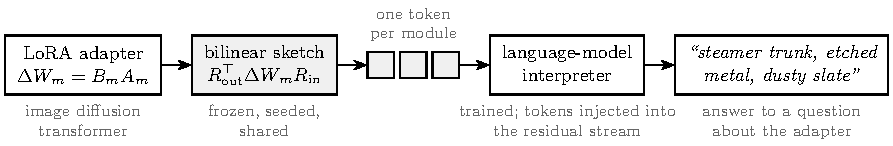
\includegraphics[width=0.88\linewidth]{figures/fig_architecture.pdf}
\caption{The diffusion adapter oracle. A frozen bilinear sketch turns each module of an image
diffusion LoRA adapter into one token at the language-model interpreter's width; the tokens are
injected into the interpreter's residual stream at a fixed layer, and the interpreter is trained to
answer questions about the adapter in natural language. Shaded parts are frozen; only the
interpreter is trained. The diffusion model is never run.}
\label{fig:architecture}
\end{figure}

The meta-model has three parts: an encoder that turns an adapter into tokens, an injection that
places those tokens in the interpreter's residual stream, and a supervision scheme
(Figure~\ref{fig:architecture}). Only the interpreter is trained.

\paragraph{Encoder.}
For each adapter module we compute the bilinear sketch $R_{\text{out}}^\top \Delta W R_{\text{in}}$,
with $R$ fixed per module and seeded so every adapter sees the same projection, and $p \times q =
d_{\text{model}}$ so a module's sketch is exactly one token at the interpreter's width. This is a
linear function of $\Delta W$, so it is invariant to the GL($r$) gauge and to coupled sign flips by
construction, with no canonicalisation step to get wrong. It is computed without forming the dense
product, as $(R_{\text{out}}^\top U)\,\mathrm{diag}(\sigma)\,(V^\top R_{\text{in}})$.

\paragraph{A projection map is unnecessary.}
A same-architecture reader can map each direction through the base model's own write-back matrix so
it lands in the reader's residual stream. We built that analogue and found it does nothing: every
module already carries one side at residual width, input-side modules on the input and output-side
modules on the output, so selecting that side by dimension leaves the map with nothing to multiply
and the measured ratio $\lVert Wd \rVert / \lVert d \rVert$ is exactly 1. Selecting the side by
module name instead, which is how our implementation began, silently discarded 42.1\% of modules.

\paragraph{Injection.}
Tokens occupy the first positions of the prompt, which are placeholders, and are added to the
embedding there, rescaled to the norm of the activation they join:
$h \leftarrow h + (\lVert h \rVert / \lVert v \rVert)\, v$.
This adds no trained parameters. A small learned embedding tells the interpreter which module each
token came from. An unnormalised version diverges, which LoRAcle also reports.

\paragraph{Supervision and interpreter.}
Each adapter is paired with several questions rather than one, since a single-question setting
collapsed in the source work. Targets are first-person descriptions of the adapter's concept. The
interpreter is Qwen3-14B with a LoRA trained at $3\times10^{-5}$. Warm-started runs inherit the warm
start's rank of 256, about $1.03\times10^{9}$ trainable parameters, because loading a released
interpreter replaces any LoRA configured beforehand; we report this because our configurations
requested smaller ranks and were silently overridden.

\section{Corpus}
\label{sec:corpus}

The method needs many adapters with known content, and an image adapter costs about forty minutes to
mint against roughly twenty seconds for a small text adapter, so the corpus is the expensive part.

We mint adapters for FLUX.2-klein-4B with ai-toolkit. Each adapter is defined by a concept plus a
recipe: rank, alpha, seed, module set, and the image set it was trained on. Concepts are
compositional, combining a family, an object, a medium and a palette; the corpus uses 128 of these
alongside 27 curated concept names, for 155 in total. Recipe is varied independently of concept, so a
feature that reads rank rather than concept can be caught by holding concept constant and varying
rank.

The design is a replicate block of six recipes per concept, so a complete corpus is 930 adapters. We
release 831, with 83 concepts at all six replicates. Held-out size is the number of concepts with at
least three adapters, so it depends on how many blocks are filled. The encoder comparison in
Section~\ref{sec:encoder} was run at 625 adapters and 120 concepts with 98 held out; the results in
Section~\ref{sec:results} at 764 and 155 with 105 held out.

\section{Which weight encoder preserves concept}
\label{sec:encoder}

Before training an interpreter we ask whether concept is recoverable from the weights, and which
encoder preserves it. Both questions have a scale, and the answers differ by scale.

Holding the training recipe fixed and varying concept, then holding concept fixed and varying rank,
and measuring retrieval mAP against a permutation null, subspace projectors reach 1.000 on the
concept axis and 0.931 on the rank axis (both $p=0.0005$), while a feature built to read only rank
stays at chance ($p=0.78$ and $p=0.92$). Concept is recoverable from weights and survives rank
variation. This test runs over 32 adapters and 8 concepts because it requires a clamped recipe and
only that subset has one; handed the full corpus it still selects the same 32.

At the interpreter's scale the ordering inverts (Figure~\ref{fig:inversion}). Fitting one
classifier per feature on the interpreter's own split (625 adapters, 98 held out, chance 0.0083),
the sketch reaches 0.092 (11.0 times chance, top-5 0.194), the singular-direction detector 0.061
(7.3 times chance), and the subspace projectors 0.031 (3.7 times chance).

\begin{figure}[t]
\centering
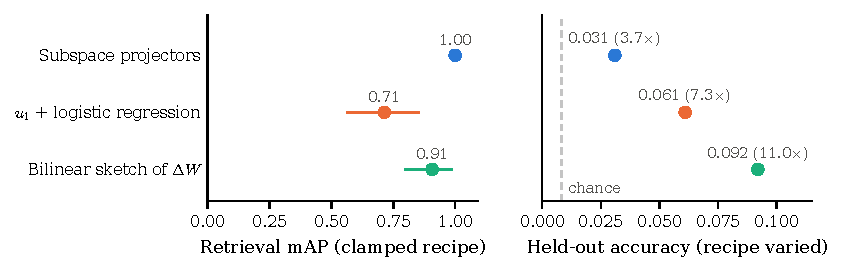
\includegraphics[width=0.80\linewidth]{figures/fig_encoder_inversion.pdf}
\caption{The encoder that wins the small clamped-recipe test loses at the scale the interpreter
operates at. Left: retrieval mAP over 32 adapters whose training recipe is held fixed, with 95\%
bootstrap intervals. Right: held-out accuracy of one linear classifier per feature over 625
adapters and 120 concepts with the recipe varied; the dashed line is chance ($1/120$). Colours
identify the same feature in both panels. Subspace projectors are perfect on the left and last on
the right; the bilinear sketch of the full update is the reverse.}
\label{fig:inversion}
\end{figure}

Subspace projectors win the clamped test outright and come last at scale. This is why
Section~\ref{sec:method} uses the sketch, and it is a caution about the smaller test, which is the
one such features are usually validated on. Training accuracy is 1.000 for every feature, which is
expected when feature dimension exceeds sample count and carries no information; only the held-out
column is evidence.

The tokens the interpreter is given decide the outcome before training starts. An earlier encoder
emitted one unit-normalised token per singular direction. Measured the same way those tokens recover
nothing, 0 of 98 at $p=1.00$, while recovering rank at 1.8 times chance from the identical tokens.
Repairing the 42.1\% module drop of Section~\ref{sec:method} moved that result from 1 of 98 to 0 of
98, so the defect was real and was not the cause.

\section{Results}
\label{sec:results}

\begin{figure}[t]
\centering
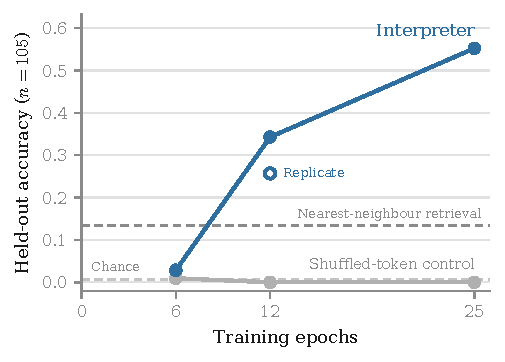
\includegraphics[width=0.66\linewidth]{figures/fig1_epoch_threshold.pdf}
\caption{Held-out accuracy rises with the training budget and has not saturated. The interpreter
reaches 2.9\%, 34.3\% and 55.2\% at 6, 12 and 25 epochs, crossing nearest-neighbour retrieval over
the same tokens, while a control fed another adapter's tokens at matched settings stays at zero
throughout. Chance is $1/155$. The open marker is an independent run of the 12-epoch configuration.
Held-out adapters are unseen adapters of training concepts, one per concept, $n=105$.}
\label{fig:epochs}
\end{figure}

\begin{table}[t]
\centering
\caption{Held-out performance by training budget. Held-out adapters are unseen adapters of concepts
that do appear in training, minted at a different rank, seed and module set. Cross-LoRA feeds a
trained interpreter a different adapter's tokens. Retrieval rank is the normalised rank of the true
concept, where 0.5 is chance and lower is better. Chance accuracy is 0.0065.}
\label{tab:main}
\begin{tabular}{lccccc}
\toprule
Configuration & Train & Held-out & $\times$chance & Cross-LoRA & Rank \\
\midrule
\textbf{25 epochs} & 0.622 & \textbf{58/105 (55.2\%)} & \textbf{85.6} & \textbf{0/105} & \textbf{0.186} \\
25 epochs, shuffled control & 0.191 & 0/105 & 0 & 0/105 & 0.482 \\
\textbf{12 epochs} & 0.589 & \textbf{36/105 (34.3\%)} & 53.1 & \textbf{0/105} & 0.270 \\
12 epochs, repeat & 0.500 & 27/105 (25.7\%) & 39.9 & 0/105 & 0.325 \\
12 epochs, shuffled control & 0.037 & 0/105 & 0 & 0/105 & 0.494 \\
12 epochs, no-injection control & 0.016 & 0/105 & 0 & 0/105 & 0.510 \\
6 epochs & 0.085 & 3/105 (2.9\%) & 4.4 & 4/105 & 0.459 \\
12 epochs, cold start, rank 16 & 0.240 & 10/105 (9.5\%) & 14.8 & 0/105 & 0.425 \\
\bottomrule
\end{tabular}
\end{table}

\paragraph{What the interpreter says.}
Held-out adapters, verbatim, from the 12-epoch configuration, given only the adapter's weights:

{\small
\begin{verbatim}
adapter: gen_object__fern_frond__etched_metal__mono_contrast
output:  "A concept adapter for gen object fern frond etched metal
          mono contrast."

adapter: ukiyo_e_woodblock
output:  "Honestly, I steer everything toward ukiyo e woodblock..."
\end{verbatim}}

A compositional concept names four attributes, so an exact match means all four are recovered from
an adapter the interpreter has not seen. The errors are structured. A typical failure returns the
subject and palette correctly and the medium wrongly (Figure~\ref{fig:slots}). Scoring each
attribute separately over the 86
compositional held-out adapters gives family 0.80, subject 0.47, palette 0.45 and medium 0.40, so
the rendering medium is what these weights encode least legibly.

\begin{figure}[t]
\centering
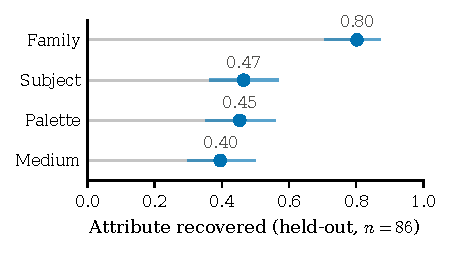
\includegraphics[width=0.44\linewidth]{figures/fig_slot_accuracy.pdf}
\caption{The concept family is recovered most often and the rendering medium least. Each
compositional concept names four attributes; a bar gives the fraction of the 86 compositional
held-out adapters whose generation contains that attribute, at 12 epochs. Family takes few values
and is easiest; medium is what these weights encode least legibly.}
\label{fig:slots}
\end{figure}

Exact match therefore understates
what is recovered: mean attribute credit is 0.427, against 0.014 when the same trained interpreter is
fed another adapter's tokens.

\paragraph{The description follows the weights.}
Both controls sit at exactly zero (Table~\ref{tab:main}). Fisher's exact test against the matched
control gives $p = 3.8\times10^{-13}$ at 12 epochs and $5.2\times10^{-23}$ at 25, and Holm correction
across the configurations tested leaves both significant. The cross-LoRA column is the sharpest form
of the check: it takes a trained interpreter and feeds it a different adapter's tokens, and accuracy
falls to zero at every budget. Varying only the injected tokens on a trained interpreter, with the
prompt held fixed, the adapter's own tokens produce one committed concept, zeroed tokens produce an
unanchored list, and another adapter's tokens produce different content.

\paragraph{It beats memorisation.}
Nearest-neighbour retrieval over the identical tokens reaches 13.3\%, against 55.2\%, Fisher
$p = 7.4\times10^{-11}$. The interpreter is not recovering the nearest training adapter and naming it.

\paragraph{The training budget is the binding constraint.}
Accuracy rises monotonically and had not saturated at the largest budget we ran
(Figure~\ref{fig:epochs}), and retrieval rank falls over the same range, 0.459 to 0.270 to 0.186
against a chance line of 0.5. Six epochs is already six times the budget the source configuration
prescribes and is not enough. Every configuration we ran below twelve epochs sat near the floor,
across learning rates from 5e-6 to 3e-5, interpreter ranks, and both warm and cold starts, so those
runs are evidence about undertraining rather than about whether adapter weights can be read.

\paragraph{Capacity contributes but is not required.}
A cold-started interpreter at rank 16, sixteen times smaller at $6.5\times10^{7}$ trainable
parameters, reaches 9.5\% at twelve epochs against its own control at zero (Fisher
$p = 7.8\times10^{-4}$), so a small interpreter does read the weights. The warm-started model is
better at the same budget, 34.3\% against 9.5\% ($p = 1.0\times10^{-5}$). That configuration varies
capacity and the warm start together and bounds their combined contribution without separating them.

Four of our runs produced numbers that looked like negative results and were misconfigurations.
Appendix~\ref{app:protocol} states the seven checks that would have caught them, each phrased as the
check rather than the failure.

\section{Limitations}

Nearly half of held-out adapters are still described wrongly, and 55.2\% is not a system to rely on
unsupervised. The result is generalisation to unseen adapters of training concepts, not to unseen
concepts: a split holding out the concept would require emitting a name the interpreter was never
trained to produce, and we do not claim that setting. Accuracy had not saturated at the largest budget we ran, so we do not know where the
curve flattens or what reaching it costs. Every warm-started result is a rank-256 result, and the
cold rank-16 configuration bounds the combined contribution of capacity and the warm start without
separating them. Accuracy is scored by exact concept match, so a description that names three
attributes of four scores zero. The clamped-recipe test of Section~\ref{sec:encoder} runs over 32
adapters and cannot be enlarged without minting a differently structured corpus. Our sketch recovers
rank at 3.8 times chance, so it is not recipe-blind. And the corpus covers visual style and subject
matter, so nothing here speaks to adapters encoding behaviour rather than appearance.

\section{Conclusion}

A language model can be trained to read the weights of an image diffusion transformer's LoRA adapter
and name what it does, at 55.2\% on held-out adapters of training concepts against 0\% for a matched
control, without ever
running the model those weights modify. The training budget rather than the architecture was the
binding constraint, and the figure is a lower bound. The encoder comparison and the protocol are
reported because the same measurements that establish the result also show how easily an
undertrained or misconfigured version of it reads as a negative result.

\bibliographystyle{plainnat}
\bibliography{refs}

\appendix
\section{Evaluating weight-space readers}
\label{app:protocol}

Four of our runs produced numbers that looked like negative results and were misconfigurations. Each
would have been read as evidence about whether adapter weights can be read. The protocol below comes
from them, and each item is stated as the check that would have caught the failure.

\begin{enumerate}\itemsep2pt
\item \textbf{Read training accuracy before held-out accuracy.} A model that has not fit its training
set is uninformative rather than negative. Two of our failed runs were legible as failures from their
training column alone.
\item \textbf{Establish a positive control before the main experiment.} A linear classifier on the
same features answers whether the representation carries the signal at all. Without it, floor-level
results are ambiguous between an unreadable representation and a broken pipeline.
\item \textbf{Match controls to the configuration they control for.} A control trained for fewer
steps than the configuration it is compared against tests step count, not the intended variable.
\item \textbf{Quote the comparison measured on the same corpus.} Our memorisation comparison scored
0.231 at 13 concepts and 0.029 at 120. A threshold carried across a corpus change measures the change.
\item \textbf{Validate a borrowed recipe's regime, not its constants.} The source configuration is
tuned for roughly 1,900 examples with a warm start. Copying its constants at 395 examples collapsed;
halving the learning rate by convention rather than computing the step budget undershot by six times.
\item \textbf{Read the artefact, not the record of what it was meant to be.} A token cap truncated by
prefix and dropped the same 34 of 50 modules from every adapter while the configuration looked
correct; a warm start silently set the interpreter rank while the saved arguments recorded the
requested one. Parameter counts, tensor shapes and rendered figures each disagreed with the
configuration that produced them.
\item \textbf{Run the cross-adapter control during training, not after it.} Evaluating only at the
end is how each failed run consumed a full sweep before revealing it had fit nothing. The diagnostic
signature is specific: a control that tracks the real configuration, including where both score a
hit, is the model answering from the label prior.
\end{enumerate}

\section{Additional detail}

\paragraph{Extraction cost.} The sketch is computed from the LoRA factors without forming
$\Delta W$, using a compact SVD of the small $r \times r$ core. Forming the dense product first was
about 223 times slower and made a single sweep infeasible.

\paragraph{Held-out splits.} Two splits are used. Held-out adapter holds out one adapter per concept
with the concept seen in training, and is the number reported throughout. Held-out family holds out
both the adapter and the concept; scoring there would require the interpreter to emit a concept name
it was never trained to produce, and we report it only for completeness.

\paragraph{Statistical procedure.} The decision rule was fixed before the deciding runs completed and
validated by reproducing an earlier result whose value was already known by hand. Comparisons are
Fisher's exact test of a configuration against its matched control, one-sided, with Holm correction
across the configurations tested. Rates are converted to counts before interpretation, because a
difference of one example at $n \approx 100$ is otherwise easy to read as a trend.

\end{document}
